\documentclass[a4 paper]{article}
% Set target color model to RGB
\usepackage[inner=2.0cm,outer=2.0cm,top=2.5cm,bottom=2.5cm]{geometry}
\usepackage{setspace}
\usepackage[rgb]{xcolor}
\usepackage{verbatim}
\usepackage{subcaption}
\usepackage{amsgen,amsmath,amstext,amsbsy,amsopn,tikz,amssymb}
\usepackage{fancyhdr}
\usepackage[colorlinks=true, urlcolor=blue,  linkcolor=blue, citecolor=blue]{hyperref}
\usepackage[colorinlistoftodos]{todonotes}
\usepackage{rotating}
\usepackage[ruled, vlined, noend]{algorithm2e}
\usepackage{wrapfig}
\usepackage{enumitem}

\usepackage{cleveref}

\usepackage{float} 
\SetKwInOut{KwParams}{Parameters}

\usepackage{minted}
\usemintedstyle{vs}
\hypersetup{%
pdfauthor={CS2420},%
pdftitle={CS2420 Programming Assignment},%
pdfkeywords={CS2420},%
pdfcreator={PDFLaTeX},%
pdfproducer={PDFLaTeX},%
}

\usepackage{booktabs}
\newcommand{\ra}[1]{\renewcommand{\arraystretch}{#1}}

\newtheorem{thm}{Theorem}[section]
\newtheorem{prop}[thm]{Proposition}
\newtheorem{lem}[thm]{Lemma}
\newtheorem{cor}[thm]{Corollary}
\newtheorem{defn}[thm]{Definition}
\newtheorem{rem}[thm]{Remark}
\numberwithin{equation}{section}

\newcommand{\homework}[7]{
   \pagestyle{myheadings}
   \thispagestyle{plain}
   \newpage
   \setcounter{page}{1}
   \noindent
   \begin{center}
   \framebox{
      \vbox{\vspace{2mm}
    \hbox to 6.28in { {\bf Harvard CS 2420:~Computing at Scale (Fall 2025) \hfill {\small (#2)}} }
       \vspace{6mm}
       \hbox to 6.28in { {\Large \hfill #1  \hfill} }
       \vspace{6mm}
       \hbox to 6.28in { {\it Instructor: {\rm #3} \hfill \textbf{Team}: {\rm #5}
       %, Harvard ID:
       {\rm #6}} }
       \hbox to 6.28in { {\hfill \it 
       %Your teammates: 
       {\rm #7}  }}
      \vspace{2mm}}
   }
   \end{center}
   \markboth{#5 -- #1}{#5 -- #1}
   \vspace*{4mm}
}

\newcommand{\problem}[2]{~\\\fbox{\textbf{Part #1}}\hfill (#2 points)\newline\newline}
\newcommand{\subproblem}[1]{~\newline\textbf{(#1)}}
\newcommand{\D}{\mathcal{D}}
\newcommand{\Hy}{\mathcal{H}}
\newcommand{\VS}{\textrm{VS}}
\newcommand{\solution}{~\newline\textbf{\textit{(Solution)}} }

\newcommand{\bbF}{\mathbb{F}}
\newcommand{\bbX}{\mathbb{X}}
\newcommand{\bI}{\mathbf{I}}
\newcommand{\bX}{\mathbf{X}}
\newcommand{\bY}{\mathbf{Y}}
\newcommand{\bepsilon}{\boldsymbol{\epsilon}}
\newcommand{\balpha}{\boldsymbol{\alpha}}
\newcommand{\bbeta}{\boldsymbol{\beta}}
\newcommand{\0}{\mathbf{0}}
\newcommand{\pya}[1]{\mintinline{python}{#1}}

\newcommand{\bigO}[1]{$\mathcal{O}(#1)$}
\newcommand{\bigo}[1]{\mathcal{O}\left(#1\right)}

\begin{document}
\homework{Problem Set 1}{Due: 09/22/2025 at 11:59PM EDT}{Professor H.T. Kung}{}
{ % your name goes here %
Alexander Ingare
zingare@g.harvard.edu
}
{}{}

\begin{center}
\textbf{Please include your full name and email address in your submission.
(See Section \ref{sec:submission})
}    
\end{center}

\section*{Introduction}
\subsection*{Assignment Objectives}
The objectives of this assignment are to:
\begin{itemize}
    \item Introduce the concept of data reuse strategies when performing computations from within a memory hierarchy. 
    \item Illustrate how outer products can be more efficient for matrix-matrix multiplication (MMM) than inner products.
    \item Demonstrate how arithmetic intensity can affect runtime. 
\end{itemize}


\subsection*{Virtual Machine Setup}
\begin{itemize}
\item If using a device with Apple Silicon (M1 and M2 laptops) please see this 
\href{https://docs.google.com/document/d/1xWgQsQKmSuJR5kxzT_85huf9Bf4HRi94qkcdeuMydJw/edit}{Google Doc} 
for virtual machine setup instructions.

\item If using a device with Intel or AMD processors (including older Macbooks from 2020 or earlier), please see this
\href{https://docs.google.com/document/d/1g_JU17qZ06vynSV1yvXgBf32fLaRqTArZO213JJtejg/edit}{Google Doc}
for virtual machine setup instructions.

\end{itemize}

\subsection*{Refresher}
\subsubsection*{Matrix-Matrix Multiplication}
We define matrix-matrix multiplication (MMM) as $C = C + A \times B$, where $A$ and $B$ are input matrices of size $M \times K$ and $K \times N$, respectively, and $C$ is the $M \times N$ result matrix.
Keep in mind that $C$ being both an input and output means elements of $C$ must be \textbf{read from the external memory} into the local memory first before being used and then written back.
For simplicity, we assume square matrices throughout this assignment (i.e., $M = N = K$). 
However, concepts and methods learned from this assignment generalize to non-square matrices.
As discussed in lecture, MMM is a fundamental operation underlying many machine learning computations. 

\subsubsection*{Arithmetic Intensity}
Arithmetic intensity ($\alpha$) is the ratio of arithmetic operations performed (or \# ops) to number of memory accesses (IO):
\[
\alpha = \frac{\#\text{ ops}}{\text{IO}}
\]
Note: we will consider IO in units of 4-byte elements (i.e., 32-bit floating point numbers).
Arithmetic intensity is an important metric because it captures how much computation may be done for each memory access.
We prefer algorithms with a high arithmetic intensity in order to minimize the IO for the same number of arithmetic operations performed.

\subsubsection*{Memory Hierarchy and Computation from Local Memory}
For simplicity, we will assume a simple memory hierarchy with 2 levels: a \textbf{fast} local SRAM and a \textbf{slow} external DRAM.
We will also assume the local memory (SRAM) is entirely user-managed (i.e., the memory does not have a built-in eviction policy).
That is, we can specify what data is held, for whatever length of time, so long as there is sufficient memory capacity.

Computations may only be performed directly on data stored in local memory, so operands (inputs and outputs to be used or written back) must be located in the local SRAM (and not the external DRAM).
For any algorithm, final results must be written back to the slower external memory (DRAM), but intermediate values can be either held in faster memory or written back to slower memory.

\subsubsection*{Analysis Details and Hints}

For our analysis, we will follow these guidelines for ease of analysis: 
\begin{itemize}
\item Individual reads and writes to external memory are considered \textbf{separate IO operations}.
\item \textbf{Initializing a variable in local memory} does not require an IO operation.
\item At the start of each question, we assume \textbf{fast memory is entirely cleared/zeroed} (all zeroes).
\item All final computed values of $C$ should be \textbf{written back to external memory} and not just kept in fast memory. (Hint: this means your IO should \textit{always} factor in at least reading and writing $C$!). 
\item Multiply-accumulates (MACs) count as \textbf{two arithmetic operations} (i.e., one multiplication followed by one addition):
\[
 z \leftarrow z + x \cdot y \text{ means } \texttt{z += x * y (C code)}
\]
\
\end{itemize}



\subsubsection*{Example: Arithmetic Intensity for Incrementing All Elements of a Vector by 1}
In the next section, we will be asking you to derive the arithmetic intensity for certain algorithms.
For each question, clearly state \textbf{where data is being moved} to/from as well as \textbf{when the data is being moved} (i.e., the order of data movement).
Describe any additional assumptions you make.
To simplify analysis, you may express your analysis on arithmetic intensity in terms of $N$.

Here is an example of how to calculate the arithmetic intensity for the following algorithm when local memory can hold only $\frac{N}{2}$ elements for an even integer $N$:\\
\begin{algorithm}[H]
\SetAlgoLined
\SetInd{0.25em}{0.5em}
\tcp{$a$ is a vector with $N$ elements}
\For{$n = 1 \to N$}{
    $a[n] \longleftarrow a[n] + 1$;
}
\caption{Vector increment}
\label{algo:vector_increment}
\end{algorithm}

We start by reading in the first $\frac{N}{2}$ elements of $a$ from slow external memory into local memory.
Next, we add 1 to the value of each element in local memory, and then write them back to external memory.
We repeat this for the last $\frac{N}{2}$ elements of $a$.
In total, we read $N$ elements from external memory and write back $N$ elements to external memory, and perform $N$ additions.
That is, we have $2N$ accesses to slow memory and $N$ operations.
As a result, our arithmetic intensity is:
\[
\alpha = \frac{N}{2N} = \frac{1}{2}
\]

\noindent

\newpage
\section{Arithmetic Intensity for an Individual Inner Product}
\label{sec:ip_ai}
An inner product (also called a dot product) between $a$ and $b$, two $N$-dimension vectors  with $a$ being a row vector and $b$ a column vector, will result in a single element, as computed by the following algorithm:

\begin{algorithm}
\SetAlgoLined
\SetInd{0.25em}{0.5em}
$sum \longleftarrow 0$;
\For{$n = 1 \to N$}{
    $sum \longleftarrow sum + a[n] \cdot b[n]$\;
}
\Return $sum$
\caption{Inner Product of Two Vectors}
\label{algo:inner-product}
\end{algorithm}

\problem{1.1}{5}
Calculate arithmetic intensity for the inner product computation (\Cref{algo:inner-product}) when local memory can hold 3 elements for the scheme where we keep $sum$, a single element of $a$, and a single element of $b$ in memory.
Reminder: initializing $sum$ to zero does not require any reads from external memory, but the final result must be written back to external memory!

\solution{1.1}

% Part 1.1
\[
\text{read } a, b \;\;\Rightarrow\; 2 \text{ IO accesses}
\]
\[
\text{sum } \;\;\Rightarrow\; \text{ No I/O accesses except for final write-back (1)}
\]
\[
\text{mul, add } \;\;\Rightarrow\; 2 \text{ Ops}
\]
\[
\alpha = \frac{2N}{2N+1}
\]

\problem{1.2}{10}
Calculate arithmetic intensity for the inner product when local memory can hold $\frac{N}{2} + 2$ elements.
(Hint: start by bringing in the first half of $b$.)

\solution{1.2}

% Part 1.2
\[
\frac{N}{2} + 2 \text{ elements } \;\;\Rightarrow\; \frac{N}{2} + 1 \text{ after local sum } \;\;\Rightarrow\; \frac{N}{2} \text{ elements from $b$, 1 element from $a$, 1 element for sum}
\]

Reading is sequential and there is no data reuse for vectors $a$ and $b$. 
\[
\therefore \alpha \text{ will remain the same}
\]
\[
\alpha = \frac{2N}{2N+1}
\]

\problem{1.3}{5}
Calculate arithmetic intensity for the inner product when local memory can hold $2N + 1$ elements.

\solution{1.3}

% Part 1.3
\[
2N+1 \text{ elements, same logic from Part 1.2}
\]
\[
\therefore \alpha \text{ will remain the same}
\]
\[
\alpha = \frac{2N}{2N+1}
\]

\newpage
\section{Arithmetic Intensity for an Individual Outer Product}
\label{sec:op_ai}
An outer product between two $N$-dimension vectors $a$ and $b$, where $a$ is a column vector and $b$ is a row vector, will result in an $N \times N$ matrix $C$.
$C = a \times b$ is computed by the following algorithm:

\begin{algorithm}
\SetAlgoLined
\SetInd{0.25em}{0.5em}
\For{$m = 1 \to N$}{
    \For{$n = 1 \to N$}{
        $C[m][n] \longleftarrow a[m] \cdot b[n]$;
    }
}
\caption{Outer Product on a Pair of Vectors}
\label{algo:outer-product}
\end{algorithm}
\noindent
Note: in this example, $C$ does not need to be fetched from external memory---we are only writing out values, \textbf{not} updating pre-existing ones.

\problem{2.1}{5}
Calculate the arithmetic intensity for the outer product computation (\Cref{algo:outer-product}) when local memory can hold 3 elements for the scheme where we hold a single element of $A$, $B$, and $C$ at a time.

\solution{2.1}

% Part 2.1

\textbf{Inner loop:} $1$ op, $2$ reads, $1$ write. 
Vector $a$ stays in memory, but vector $b$ has $N-1$ more reads. 

\medskip
\textbf{Outer loop:} $N^2$ ops, $N^2$ writes to external memory, 
$N$ reads for vector $a$, $N^2$ reads for vector $b$.

\[
\Rightarrow \;\; \alpha = \frac{N^2}{2N^2 + N}
\;\;\;\Rightarrow\;\;\;
\alpha = \frac{N}{2N+1}
\]

\problem{2.2}{10}
Calculate the arithmetic intensity for the outer product when local memory can hold $\frac{N}{2} + 2$ elements, using the scheme where we hold half of $B$, and a single element of $A$ and $C$ in memory.

\solution{2.2}

% Part 2.2
\[
N^2 \text{ ops}, \quad N^2 \text{ writes to external memory}, \quad 
1 \text{ element of } a \quad \& \quad \tfrac{N}{2} \text{ elements of } b \text{ loaded}
\]

After loading half of $b$, cycle through $a$, do ops, load second half of $b$, 
cycle through $a$ again, do ops.

\[
\Rightarrow \alpha = \frac{N^2}{N^2 + 2N + N}
= \frac{N^2}{N^2 + 3N}
\Rightarrow \alpha = \frac{N}{N+3}
\]

\problem{2.3}{5}
Calculate the arithmetic intensity for the outer product when local memory can hold $2N + 1$ elements, using the scheme where we hold $A$ and $B$ in local memory and write the computed values of $C$ to external memory.

\solution{2.3}

% Part 2.3
$2N+1$ is max data reuse $\;\Rightarrow\;$ load all elements of vector $a$ ($N$), 
vector $b$ ($N$), $1$ element $c$ ($1$) $\;\Rightarrow\; 2N+1$.

\[
\Rightarrow \text{Total reads is } 2N, \quad 
\text{total writes is } N^2, \quad 
\text{total ops } = N^2
\]

\[
\Rightarrow \alpha = \frac{N^2}{N^2 + 2N} 
\;\;\Rightarrow\;\; 
\alpha = \frac{N}{N+2}
\]


\newpage
\section{MMM Runtimes}
\label{sec:eval}
In this section you will implement MMM with both inner and outer products, execute the code on your computer or VM and report their runtimes.

\subsection*{Implementing Inner Product MMM}
\problem{3.1}{10}
Implement inner product MMM in the function \texttt{inner\_product\_mmm()} contained in \texttt{pset1.cpp}, as described by the following algorithm:
\begin{algorithm}
\SetAlgoLined
\SetInd{0.25em}{0.5em}
\For{$m = 1 \to M$}{
    \For{$n = 1 \to N$}{
        \For{$k = 1 \to K$}{
            $C[m][n] \longleftarrow C[m][n] + A[m][k] \cdot B[k][n]$\;
        }
    }
}
\caption{Inner product MMM}
\label{algo:naivemm-mnk}
\end{algorithm}

\subsection*{Implementing Outer Product MMM}
\problem{3.2}{10}
Implement outer product MMM in the function \texttt{outer\_product\_mmm()} contained in \texttt{pset1.cpp}, as described by the following algorithm:

\begin{algorithm}[H]
\SetAlgoLined
\SetInd{0.25em}{0.5em}
\For{$k = 1 \to K$}{
    \For{$m = 1 \to M$}{
        \For{$n = 1 \to N$}{
            $C[m][n] \longleftarrow C[m][n] + A[m][k] \cdot B[k][n]$\;
        }
    }
}
\caption{Outer product MMM}
\label{algo:naivemm-kmn}
\end{algorithm}

\subsection*{Timing}
\problem{3.3}{15}
With your implementation of the MMM functions, run the provided code.
Plot the run time results, taking the average over 5 runs.
As mentioned earlier, use only square matrices (i.e., $M = N = K$) to simplify timing comparisons.
The Y-axis should be the run time (in nanoseconds) and X-axis should be the matrix dimension $N$.
Be sure to appropriately label your generated plot with axes, title, and legend.
Your plot must include data for following values of $N$: 16, 32, 64, 128, 256, 512, 1024 (every power of 2 between $2^4$ and $2^{10}$, inclusive).
For plotting, use Python’s \texttt{matplotlib}.
What trends do you observe?
Does anything stand out or seem unusual?

\solution{3.3}

% In preamble:
% \usepackage{graphicx}
% \usepackage{enumitem}

\subsection*{1. Inner Product MMM (blue):}
\begin{itemize}[noitemsep]
    \item Runtime grows steeply as $N$ increases.
    \item The algorithm computes each element ($C[m][n]$) independently, repeatedly scanning through a full row of (A) and a full column of (B).
    \item Because matrices are stored in row-major order, accessing columns of (B) causes strided, cache-unfriendly memory accesses.
    \item Each element of (A) and (B) ends up being reloaded many times, leading to high memory traffic and poor cache reuse.
\end{itemize}

\subsection*{2. Outer Product MMM (red):}
\begin{itemize}[noitemsep]
    \item Runtime increases more smoothly and consistently with $N$.
    \item The algorithm processes one index ($k$) at a time, reusing the entire column ($A[:,k]$) and row ($B[k,:]$) across all of (C).
    \item This ordering maximizes data reuse: once ($A[m][k]$) and ($B[k][n]$) are loaded, they are used in $\mathcal{O}(N)$ updates before being evicted from cache.
    \item Access patterns align well with row-major storage (especially for (B)), resulting in much higher cache efficiency.
\end{itemize}

\subsection*{3. Comparison Plot:}
\begin{itemize}[noitemsep]
    \item Outer product MMM is consistently faster than inner product MMM for all matrix sizes.
    \item The performance gap widens as $N$ grows, because cache effects dominate at large sizes.
    \item Both algorithms are $\mathcal{O}(N^3)$, but the loop order determines arithmetic intensity and cache behavior, which is why runtime differs so significantly.
\end{itemize}


\noindent\textbf{Trend:} Both implementations scale as $\mathcal{O}(N^3)$, but outer product achieves much better constant factors due to memory reuse.  \\


\noindent\textbf{Unusual Point:} The dramatic slowdown of the inner product implementation at large $N$ highlights that loop ordering and memory hierarchy effects dominate performance, even when the arithmetic work is identical.  \\

\noindent From the timing plots, outer product MMM outperforms inner product MMM because its loop ordering maximizes data reuse and cache locality. Inner product, by contrast, repeatedly reloads matrix elements due to strided memory access patterns.  

\begin{figure}[htbp!]
    \centering
    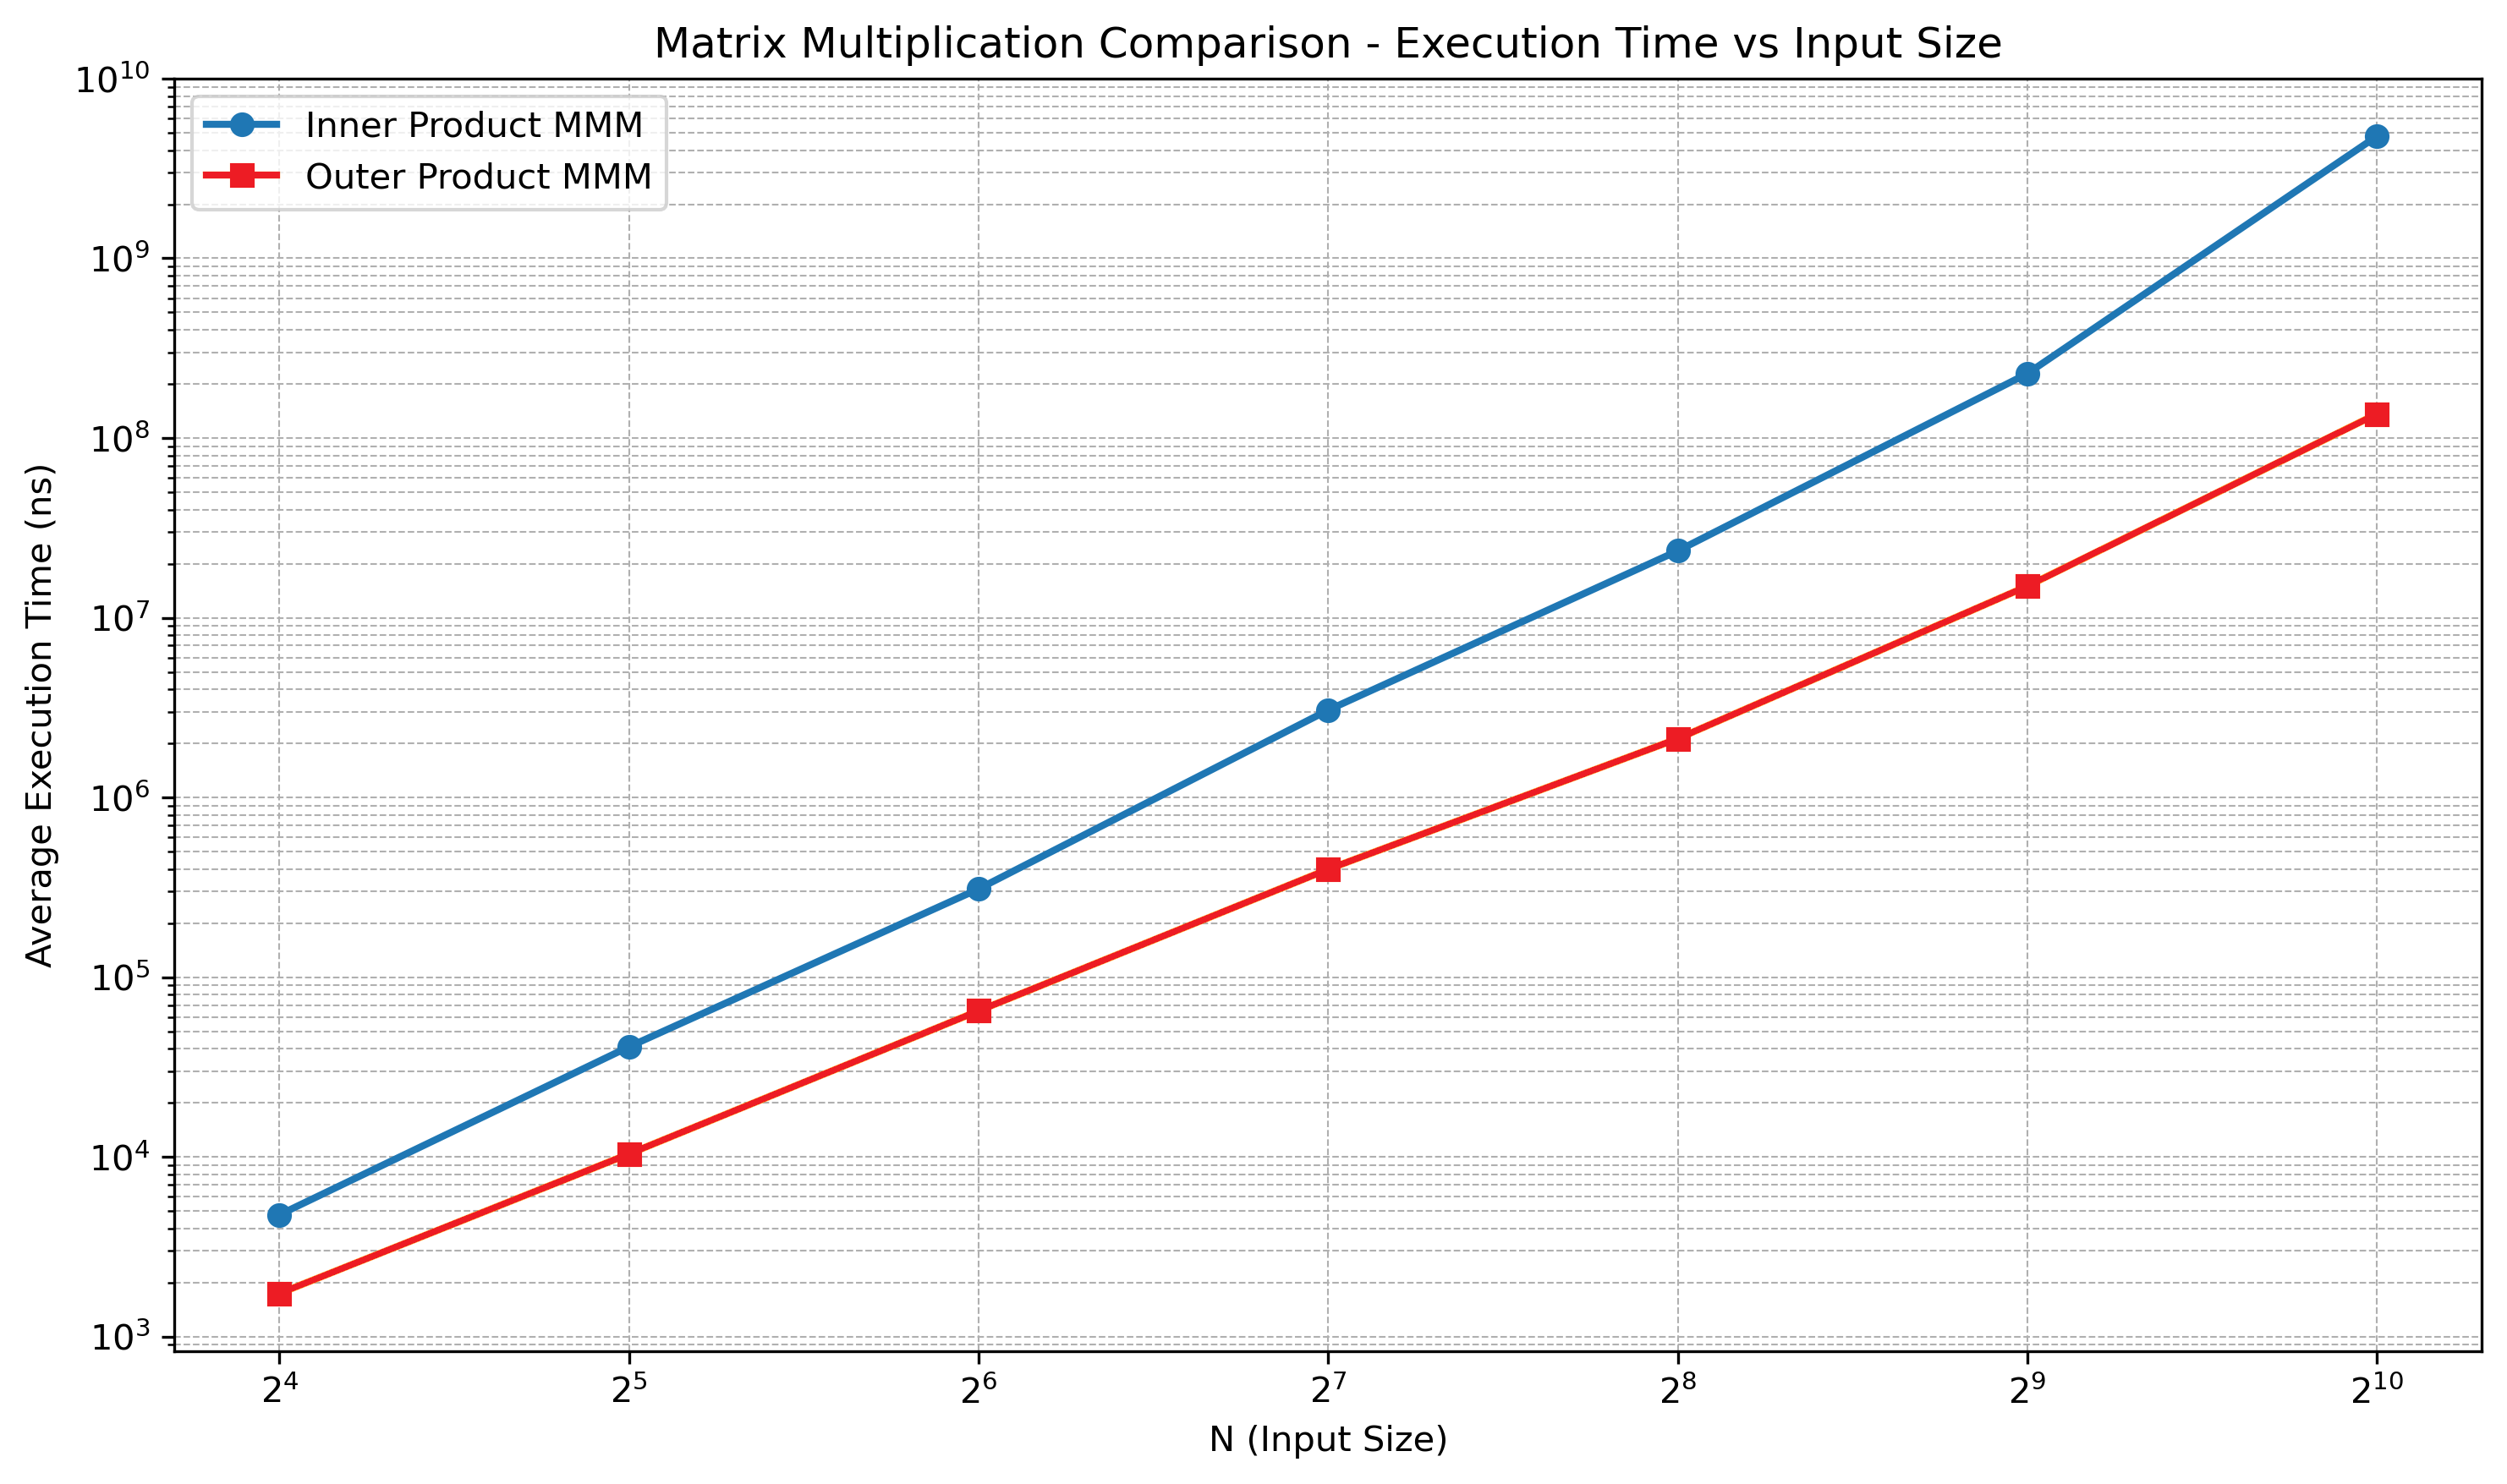
\includegraphics[width=0.9\textwidth]{matrix_multiplication_comparison.png}
    \caption{Comparison Plot: Inner vs Outer Product MMM Execution Time}
\end{figure}

\begin{figure}[htbp!]
    \centering
    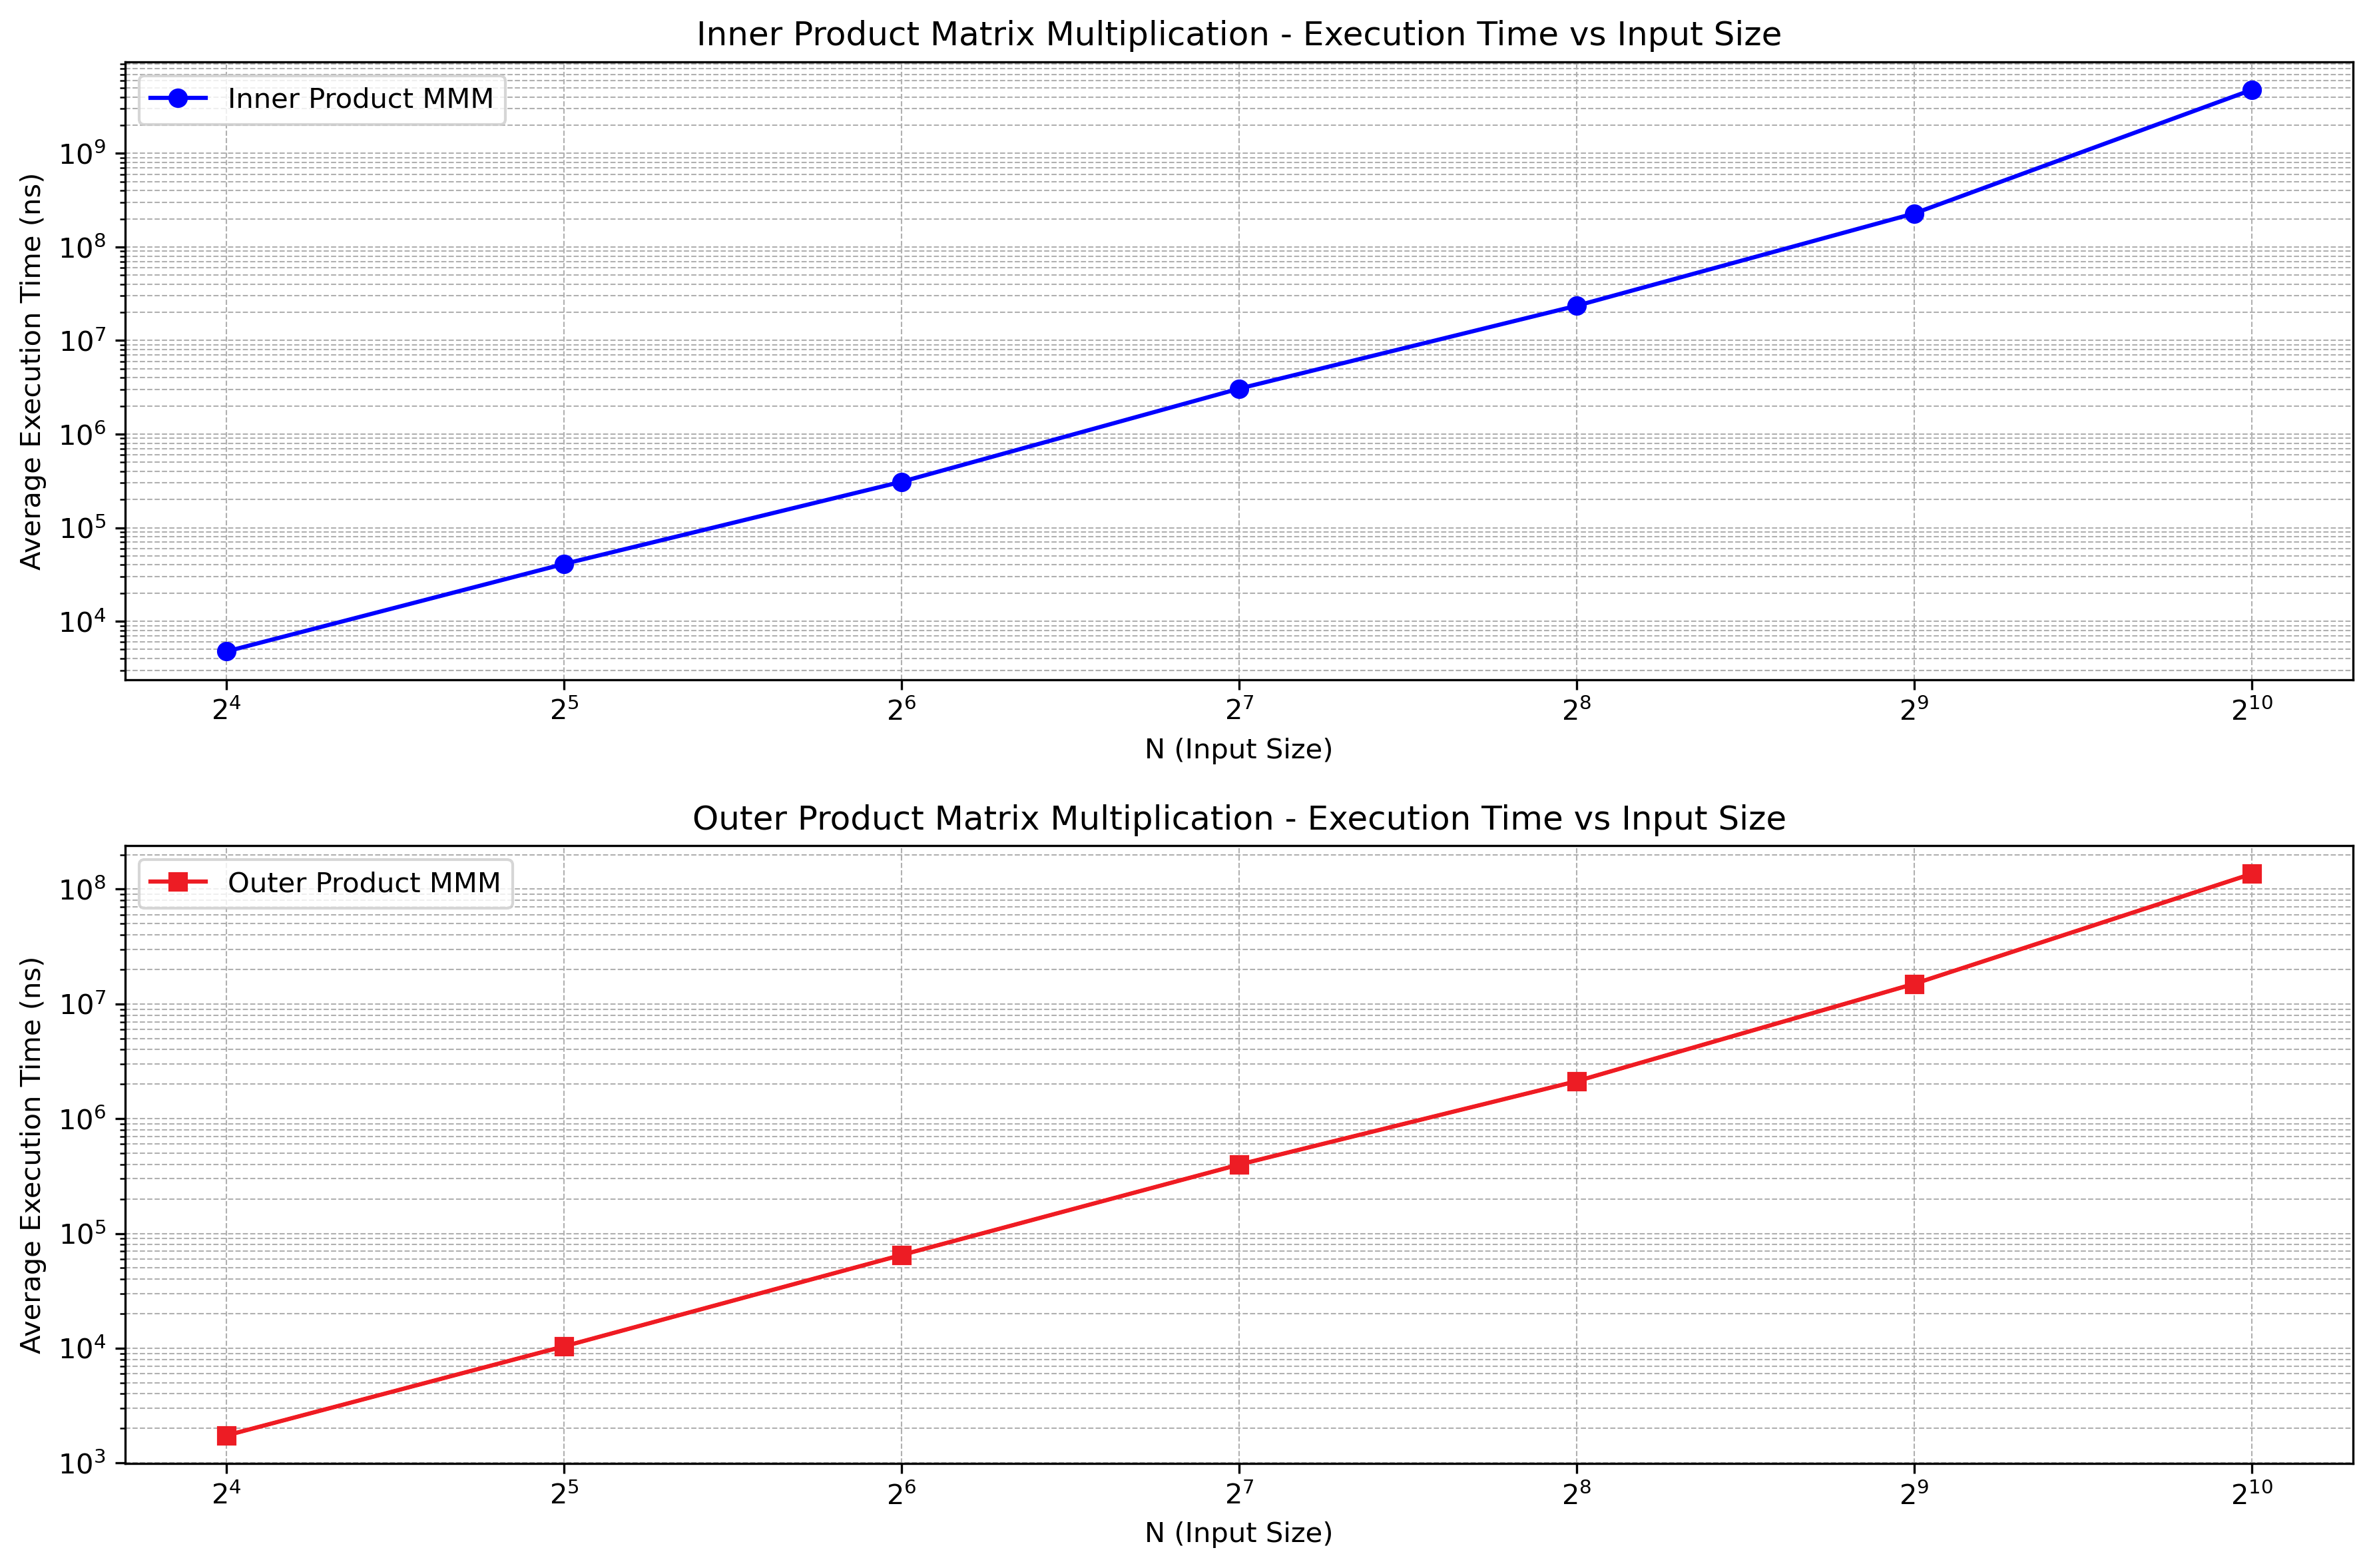
\includegraphics[width=0.9\textwidth]{matrix_multiplication_subplots.png}
    \caption{Inner/Outer Product Matrix Multiplication Execution Time vs Input Size}
\end{figure}

\pagebreak
\newpage
\section{CNN Forward Pass and Backpropagation}
\label{sec:cnn}

In this section, you will perform a complete forward pass of a convolutional neural network (CNN) and execute backpropagation for the fully connected layer at the end.

\subsection*{Background}
The CNN architecture is as follows:

\begin{itemize}
    \item \textbf{Input Image}: A $4 \times 4$ grayscale image with a single channel.
    \item \textbf{Convolution Layer}: 2 filters ($3 \times 3$) with stride 1 and no padding. No bias is considered in the convolution layer.
    \item \textbf{Activation Function}: ReLU.
    \item \textbf{Pooling Layer}: $2 \times 2$ max-pooling with stride 2.
    \item \textbf{Fully Connected Layer}: The flattened output of the pooling layer is connected to a fully connected layer with 2 output units.
\end{itemize}

Below is the input image, the filters and other setups provided for the CNN:

\begin{itemize}
    \item \textbf{Input Image (I)}, \textbf{Filter 1 (F1)}, and \textbf{Filter 2 (F2)}:
    \[
    \begin{aligned}
    I &= \begin{bmatrix}
    2 & 0 & 1 & 3 \\
    1 & 2 & 0 & 1 \\
    3 & 2 & 1 & 0 \\
    0 & 1 & 3 & 2
    \end{bmatrix}
    \quad &
    F1 &= \begin{bmatrix}
    1 & 0 & -1 \\
    0 & 1 & 0 \\
    -1 & 0 & 1
    \end{bmatrix}
    \quad &
    F2 = \begin{bmatrix}
    0 & 1 & 0 \\
    1 & -1 & 1 \\
    0 & 1 & 0
    \end{bmatrix}
    \end{aligned}
    \]

    \item \textbf{Fully Connected Weights (W\_fc)} and \textbf{Fully Connected Bias (b\_fc)}:
    \[
    \begin{aligned}
    W_{fc} &= \begin{bmatrix}
    0.2 & -0.5 \\
    -0.3 & 0.4
    \end{bmatrix}
    \quad &
    b_{fc} &= \begin{bmatrix}
    0.1 \\
    -0.2
    \end{bmatrix}
    \end{aligned}
    \]

    \item \textbf{Target Labels (Y)}:
    \[
    Y = \begin{bmatrix}
    1 \\ 0
    \end{bmatrix}
    \]
\end{itemize}


\problem{4.1}{5}

\noindent1. \textbf{Convolution}: Perform the convolution operation between the input image $I$ and both filters $F1$ and $F2$, using stride 1 and no padding. Calculate the output feature maps for each filter.
    \begin{itemize}
        \item Show step-by-step convolution calculation for both feature maps.
    \end{itemize}

\noindent2. \textbf{Activation (ReLU)}: Apply the ReLU activation function to the convolution results. Replace any negative values in the feature maps with zero.
    \begin{itemize}
        \item Write the resulting activated feature maps after applying ReLU.
    \end{itemize}

\solution{4.1.1}

\[
I =
\begin{bmatrix}
2 & 0 & 1 & 3 \\
1 & 2 & 0 & 1 \\
3 & 2 & 1 & 0 \\
0 & 1 & 3 & 2
\end{bmatrix},
\quad
\textcolor{red}{F_1} =
\begin{bmatrix}
1 & 0 & -1 \\
0 & 1 & 0 \\
-1 & 0 & 1
\end{bmatrix},
\quad
\textcolor{blue}{F_2} =
\begin{bmatrix}
0 & 1 & 0 \\
1 & -1 & 1 \\
0 & 1 & 0
\end{bmatrix}
\]

\[
\color{red}{F_{1,\text{output}} =
\begin{bmatrix}
1 & -5 \\
6 & 3
\end{bmatrix}},
\quad
\color{blue}{F_{2,\text{output}} =
\begin{bmatrix}
1 & 5 \\
5 & 4
\end{bmatrix}}
\]

\[
\begin{bmatrix}
2 & 0 & 1 \\
1 & 2 & 0 \\
3 & 2 & 1
\end{bmatrix}
\Rightarrow
\color{red}{2+0-1+0+2+0-3+0+1=1}
\quad
\color{blue}{0+0+0+1-2+0+0+2+0=1}
\]

\[
\begin{bmatrix}
0 & 1 & 3 \\
2 & 0 & 1 \\
2 & 1 & 0
\end{bmatrix}
\Rightarrow
\color{red}{0+0-3+0+0+0-2+0+0=-5}
\quad
\color{blue}{0+1+0+2+0+1+0+1+0=5}
\]

\[
\begin{bmatrix}
1 & 2 & 0 \\
3 & 2 & 1 \\
0 & 1 & 3
\end{bmatrix}
\Rightarrow
\color{red}{1+0+0+0+2+0+0+0+3=6}
\quad
\color{blue}{0+2+0+3-2+1+0+1+0=5}
\]

\[
\begin{bmatrix}
2 & 0 & 1 \\
1 & 2 & 0 \\
3 & 2 & 1
\end{bmatrix}
\Rightarrow
\color{red}{2+0-1+0+1+0-1+0+2=3}
\quad
\color{blue}{0+0+0+2-1+0+0+3+0=4}
\]

\solution{4.1.2}

\[
\textcolor{red}{F_{1,\text{output}} =
\begin{bmatrix}
1 & -5 \\
6 & 3
\end{bmatrix}}
\quad
\xrightarrow{\;\text{ReLU}\;}
\quad
\textcolor{red}{
\begin{bmatrix}
1 & 0 \\
6 & 3
\end{bmatrix}}
\]

\[
\textcolor{blue}{F_{2,\text{output}} =
\begin{bmatrix}
1 & 5 \\
5 & 4
\end{bmatrix}}
\quad
\xrightarrow{\;\text{ReLU}\;}
\quad
\textcolor{blue}{
\begin{bmatrix}
1 & 5 \\
5 & 4
\end{bmatrix}}
\]

\problem{4.2}{5}

1. \textbf{Max-Pooling}: Apply a $2 \times 2$ max-pooling operation with stride 2 to the activated feature maps from both filters. This step reduces the size of the feature maps. No padding is applied for the max-pooling layer.
    \begin{itemize}
        \item Compute the max-pooled feature maps for both activated feature maps
        \item Write down the resulting pooled feature maps.
    \end{itemize}

\solution{4.2}

\begin{align*}
\text{Max pooled for } 
\begin{bmatrix} 1 & 0 \\ 6 & 3 \end{bmatrix} & = [6] \\[6pt]
\text{Max pooled for } 
\begin{bmatrix} 1 & 5 \\ 5 & 4 \end{bmatrix} & = [5]
\end{align*}

\problem{4.3}{10}

\noindent1. \textbf{Flattening}: Flatten the output of the pooling layer into a single vector to be fed into the fully connected layer.
    \begin{itemize}
        \item Write the flattened vector.
    \end{itemize}

\noindent2. \textbf{Fully Connected Layer}: Using the weights $W_{fc}$ and bias $b_{fc}$, compute the output of the fully connected layer by applying the following equation:
    \[
    Z_{fc} = W_{fc} \cdot X_{flat} + b_{fc}
    \]
    where $X_{flat}$ is the flattened vector from the pooling layer.
    \begin{itemize}
        \item Compute the output of the fully connected layer (before applying softmax).
    \end{itemize}

\solution{4.3}

The flattened vector is 
\[
\begin{bmatrix} 6 \\ 5 \end{bmatrix}
\]

\[
Z_{fc} = W_{fc} \cdot x_{\text{flat}} + b_{fc}
\]

\[
Z_{fc} =
\begin{bmatrix}
0.2 & -0.5 \\
-0.3 & 0.4
\end{bmatrix}
\begin{bmatrix}
6 \\ 5
\end{bmatrix}
+
\begin{bmatrix}
0.1 \\ -0.2
\end{bmatrix}
=
\begin{bmatrix}
0.2 \cdot 6 + (-0.5) \cdot 5 + 0.1 \\
-0.3 \cdot 6 + 0.4 \cdot 5 - 0.2
\end{bmatrix}
\]

\[
=
\begin{bmatrix}
1.2 - 2.5 + 0.1 \\
-1.8 + 2.0 - 0.2
\end{bmatrix}
=
\begin{bmatrix}
-1.2 \\ 0
\end{bmatrix}
\]


\problem{4.4}{20}

1. \textbf{Softmax Activation}: Apply the softmax activation function to the output of the fully connected layer to get the predicted probabilities $P$. Write your answer to the nearest three decimal places. Rounding or truncating is fine. Please keep this in mind for all future parts of this problem too.
    \begin{itemize}
        \item Compute the softmax function for the output vector $Z_{fc}$.
    \end{itemize}

2. \textbf{Loss Calculation (Cross-Entropy)}: Using the provided target labels $Y$, compute the cross-entropy loss $L$ between the predicted probabilities $P$ and the true labels.
    \begin{itemize}
        \item Write down the cross-entropy loss.
    \end{itemize}

3. \textbf{Backpropagation}: Perform one round of backpropagation on the fully connected layer using the cross-entropy loss. Compute the gradients of the loss with respect to the weights $W_{fc}$, the bias $b_{fc}$, and the input vector $X_{flat}$.
    \begin{itemize}
        \item (a) Compute the gradient of the loss with respect to the output of the fully connected layer ($dZ_{fc}$).
        \item (b) Compute the gradient with respect to the weights $W_{fc}$, the bias $b_{fc}$, and the input $X_{flat}$.
    \end{itemize}

\subsection*{Solution Guidelines}
For the convolution, use the discrete convolution formula:
\[
(I * F)(i, j) = \sum_{m=0}^{2} \sum_{n=0}^{2} I(i+m, j+n) \cdot F(m, n)
\]

Apply ReLU by replacing negative values with 0.

For max-pooling, take the maximum value in each $2 \times 2$ window of the feature maps.\newline

The softmax function is given by:
\[
\text{softmax}(z_i) = \frac{e^{z_i}}{\sum_j e^{z_j}}
\]

The cross-entropy loss is:

\[
L = -\sum_{i} y_i \log(p_i)
\]

where $y_i$ is the true label and $p_i$ is the predicted probability from softmax.


\solution{4.4.1}


Softmax definition:
\[
\text{softmax}(z_i) = \frac{e^{z_i}}{\sum_j e^{z_j}}
\]

\[
\text{softmax}(Z_{fc}) = \text{softmax}
\begin{bmatrix}
-1.2 \\ 0
\end{bmatrix}
=
\begin{bmatrix}
\frac{e^{-1.2}}{e^{-1.2} + e^0} \\
\frac{e^{0}}{e^{-1.2} + e^0}
\end{bmatrix}
=
\begin{bmatrix}
0.231475 \\ 0.768524
\end{bmatrix}
\]
\solution{4.4.2}

Target label:
\[
Y = \begin{bmatrix} 1 \\ 0 \end{bmatrix}
\]

Cross-entropy loss:
\[
L = - \sum_i y_i \log_2(p_i) 
= - \log_2(0.231) 
= 1.465
\]
\solution{4.4.3}

Backpropagation:
\[
P = \begin{bmatrix} 0.231 \\ 0.769 \end{bmatrix},
\quad Y = \begin{bmatrix} 1 \\ 0 \end{bmatrix}
\]

\[
dZ_{fc} = P - Y 
= \begin{bmatrix} -0.769 \\ 0.769 \end{bmatrix}
\]

\[
dW_{fc} = dZ_{fc} \cdot x_{\text{flat}}^T 
= 
\begin{bmatrix}
-0.769 \\ 0.769
\end{bmatrix}
\begin{bmatrix}
6 & 5
\end{bmatrix}
=
\begin{bmatrix}
-4.611 & -3.843 \\
4.611 & 3.843
\end{bmatrix}
\]

\[
db_{fc} = dZ_{fc} =
\begin{bmatrix}
-0.769 \\ 0.769
\end{bmatrix}
\]

\[
dX_{\text{flat}} = W_{fc}^T \cdot dZ_{fc} =
\begin{bmatrix}
0.2 & -0.3 \\
-0.5 & 0.4
\end{bmatrix}^T
\begin{bmatrix}
-0.769 \\ 0.769
\end{bmatrix}
=
\begin{bmatrix}
0.2 & -0.5 \\
-0.3 & 0.4
\end{bmatrix}
\begin{bmatrix}
-0.769 \\ 0.769
\end{bmatrix}
=
\begin{bmatrix}
-0.385 \\ 0.692
\end{bmatrix}
\]


\newpage
\section{SIMD}
\label{sec:simd}

SIMD (Single Instruction, Multiple Data) is a technique used to improve the performance of computationally intensive tasks by performing the same operation on multiple data points simultaneously. In this question, you will explore how SIMD can be applied to matrix multiplication, a core operation you've worked with earlier in this assignment.

\problem{5.1}{25}

Consider a typical system with 512-bit SIMD registers that can hold 16 single-precision floating-point numbers. You are implementing matrix multiplication C = A * B, where A, B, and C are 1024 x 1024 matrices.

\begin{enumerate}
    \item  Describe a SIMD-based algorithm for this matrix multiplication that maximizes data reuse. Include details on data layout and access patterns. (20 points)
    \item  Calculate the theoretical speed-up of your SIMD implementation compared to a scalar version. Then, explain why the actual speed-up is likely to be lower, considering memory bandwidth limitations and cache behavior. (5 points)
\end{enumerate}

\solution{5.1}

\subsection*{(1) SIMD-Based Matrix Multiplication Algorithm}

A SIMD-based algorithm that maximizes data reuse for square matrix multiplication can be described as follows:

\begin{itemize}
    \item Since $16$ single-precision floating-point numbers fit into a 512-bit SIMD register, the tiles are chosen to be $16$ elements wide.
    \item The $1024 \times 1024$ matrices are split into $64 \times 64$ tiles, each consisting of sub-blocks that align with the SIMD width.
    \item The major ordering of the matrices is chosen to ensure unit-stride access within tiles:
    \begin{itemize}
        \item Following the standard $i$--$j$--$k$ ordering in the product
        \[
            C[i,j] \; += \; A[i,k] \times B[k,j],
        \]
        matrix $A$ should be stored in \textbf{row-major} order (contiguous rows),
        while matrix $B$ should be stored in \textbf{column-major} order (contiguous columns).
    \end{itemize}
    \item With this layout, the algorithm computes partial dot products of
    \textit{rows from a tile of $A$} with \textit{columns from a tile of $B$}.
\end{itemize}

\subsection*{Algorithm Steps}
For each matching pair of tiles from $A$ and $B$ along the shared dimension ($k$):
\begin{enumerate}
    \item Keep the $B$ tile resident in cache, since it will be reused by all rows of $A$'s tile.
    \item Stream rows of the $A$ tile one at a time:
    \begin{enumerate}
        \item Load the current row from $A$’s tile (unit-stride contiguous load).
        \item Vectorize across $C$’s columns; for each column of the $B$ tile:
        \begin{enumerate}
            \item Load the column from $B$’s tile (unit-stride contiguous load).
            \item Multiply the row of $A$’s tile with the column of $B$’s tile.
            \item Accumulate the result into the corresponding positions of the $C$ tile.
        \end{enumerate}
        \item Once the row has been used with all columns of the $B$ tile, discard it (it will not be needed again for this $k$ panel).
    \end{enumerate}
    \item Repeat the process for all rows of $A$’s tile.
    \item After all $k$ tile pairs are processed, the $C$ tile is fully accumulated and the completed tile is written back to memory once.
\end{enumerate}



\begin{algorithm}[H]
\caption{Tiled MMM with Row-Streaming (A row-major) and Column-Reuse (B column-major)}
\label{alg:tiled-mmm}
\DontPrintSemicolon
\KwIn{Matrices $A\in\mathbb{R}^{M\times K}$ (row-major), $B\in\mathbb{R}^{K\times N}$ (column-major)}
\KwOut{$C \gets A B \in\mathbb{R}^{M\times N}$}
\KwParams{Tile sizes $T_M, T_N, T_K$ (\emph{e.g.} $T_M=T_N=64$, $T_K=16$)}

\For{$mm \gets 0 \;\mathbf{to}\; M-1 \;\mathbf{step}\; T_M$}{
  \For{$nn \gets 0 \;\mathbf{to}\; N-1 \;\mathbf{step}\; T_N$}{
    \tcp{Accumulate one $T_M \times T_N$ tile of $C$}
    \For{$KB \gets 0 \;\mathbf{to}\; K-1 \;\mathbf{step}\; T_K$}{
      \tcp{Keep $B$'s tile warm: reused by all rows of $A$'s tile}
      \For{$m \gets mm \;\mathbf{to}\; mm+T_M-1$}{
        \tcp{Stream one \emph{row} from $A$'s tile (contiguous load)}
        $a\_row \gets A[m,\; KB{:}KB+T_K-1]$\;
        
        \For{$n \gets nn \;\mathbf{to}\; nn+T_N-1$}{
          \tcp{Load one \emph{column} from $B$'s tile (contiguous load)}
          $b\_col \gets B[KB{:}KB+T_K-1,\; n]$\;
          \tcp{SIMD FMA across the $T_K$ panel}
            $C[m,n] \gets C[m,n] + A[m,k] \times B[k,n]$\;        }
        \tcp{Row $m$ is fully used with this $B$ tile and can be discarded}
      }
    }
    \tcp{Write back the completed $C$ tile once}
  }
}
\end{algorithm}

\subsection*{(2) Theoretical and Practical Speedup}

\textbf{Theoretical speedup:} 
A 512-bit SIMD register holds 16 single-precision floating-point values. In an idealized kernel, each SIMD instruction performs 16 multiplies and adds in parallel, compared to a scalar kernel performing 1. Therefore, the theoretical compute speedup is approximately $16\times$.\\


\noindent\textbf{Why the actual speedup is smaller:}

\begin{enumerate}
    \item \textbf{Memory bandwidth ceiling:} Even with tiling, each panel of $A$ and $B$ must be streamed from memory and $C$ must be written back. When the required throughput to feed the FMAs exceeds available DRAM or cache bandwidth, the performance is capped well below the compute peak. In roofline terms, sustained FLOP/s is limited as follows:
    \[
      \text{sustained FLOP/s} \;\leq\; \text{bandwidth} \times \text{arithmetic intensity}.
    \]
    \item \textbf{Cache capacity and behavior:} If the working set of tiles (panels of $A$ and $B$, along with the live block of $C$) does not fit in the caches, lines are evicted and re-fetched. This increases memory traffic and reduces the reuse that the SIMD width is meant to exploit.
    \item \textbf{Vector overheads and utilization loss:} Real implementations incur extra operations such as broadcasts, shuffles, loop control, handling of non-multiples of the SIMD width, and alignment adjustments. In addition, dependency chains in accumulation can reduce instruction-level parallelism. These factors lower the effective SIMD utilization compared to the ideal case where all 16 lanes perform useful work each cycle.
\end{enumerate}


\problem{5.2}{15}

Consider a typical system with 512-bit SIMD registers that can hold 16 single-precision floating-point numbers. You are optimizing the 3D convolution operation in the CNN forward pass (ref. lec-2 p16-22) using SIMD instructions.

\begin{enumerate}
    \item Propose a SIMD-based approach for the 3D convolution operation that maximizes data reuse. Include details on data layout and access patterns. (Assume the input and filter sizes are much larger than a single SIMD register can hold, and that the stride size matches the filter size.) (10 points)
    \item One of your colleagues suggests using a SIMD width of 2048 bits to further improve performance. Explain the potential drawbacks of this approach, considering aspects such as power consumption, chip area, and applicability to other operations in CNN computation. (5 points)
\end{enumerate}

\solution{5.2}

\paragraph{(1) SIMD-based approach maximizing data reuse:}
We can express the 3D convolution as a matrix multiplication after applying the \texttt{im2col} transform. Using the indexing
\[
C[m,n] \;+=\; A[n,k] \times B[k,m],
\]
the following mapping applies:

\begin{itemize}
  \item \textbf{im2col transform:}
  \begin{itemize}
    \item The input of size $C \times H_c \times W_c$ is unrolled into
    \[
      A \in \mathbb{R}^{N \times K},
    \]
    where $N = H_o \times W_o$ is the number of sliding windows and $K = C \times H_F \times W_F$ is the flattened receptive field dimension.
    \item Each filter of size $C \times H_F \times W_F$ is flattened into a row of
    \[
      B \in \mathbb{R}^{K \times M},
    \]
    where $M$ is the number of filters.
    \item The output matrix is
    \[
      C \in \mathbb{R}^{M \times N}.
    \]
  \end{itemize}

  \item \textbf{Data layouts:}
  \begin{itemize}
    \item $A$ stored \textbf{row-major} with stride-1 along $k$ (each row corresponds to an output position $n$, contiguous in $k$).
    \item $B$ stored \textbf{column-major} with stride-1 along $k$ (each column corresponds to a filter $m$, contiguous in $k$).
    \item $C$ stored row-major.
  \end{itemize}

  \item \textbf{SIMD mapping and tiling:}
  \begin{itemize}
    \item With 512-bit SIMD, each register holds 16 FP32 values. Choose tile sizes $T_M$ and $T_N$ in multiples of 16, with $K$ split into panels of $T_K$.
    \item For each tile of $C$:
      \begin{enumerate}
        \item Stream one row of $A$ (indexed by $n$) across the $k$-panel.
        \item Reuse the corresponding panel of $B$’s columns (indexed by $m$).
        \item For each $k$ in the panel, broadcast $A[n,k]$ into a SIMD register and multiply with the 16-wide contiguous vector $B[k, m:m+15]$.
        \item Accumulate results into the $C[m:m+15,n]$ registers.
      \end{enumerate}
    \item The row of $A$ is discarded once it has been used with all columns of $B$. Each column of $B$ is reused across all rows of $A$ in the tile. The $C$ tile is written back once after all $k$-panels are processed.
  \end{itemize}
\end{itemize}

\paragraph{(2) Drawbacks of a 2048-bit SIMD width:}
\begin{itemize}
  \item \textbf{Power and area overhead:} A 2048-bit SIMD unit is larger and consumes more power, which may reduce efficiency.
  \item \textbf{Utilization waste:} If $M$ or $N$ is not a multiple of 64, many lanes will be idle and cycles are wasted.
  \item \textbf{Limited benefit across CNN layers:} Wider SIMD is not always helpful for non-GEMM layers such as pooling or activation functions, where the operation is not naturally vector-wide.
\end{itemize}


\problem{5.3}{5}

Your SIMD-optimized matrix multiplication code from Part 5.1 runs slower on a new CPU architecture with the same SIMD width but double the clock speed. Identify three possible reasons for this performance degradation and briefly explain how you would diagnose each issue.


\solution{5.3}\\

\noindent Although the algorithm maximizes data reuse through row-streaming of $A$ and reuse of columns from $B$, performance may still degrade on a newer CPU with higher clock frequency but the same SIMD width:

\begin{enumerate}
    \item \textbf{Smaller caches in the new architecture:}  
    The algorithm depends on keeping the tile of $B$ resident in cache while streaming rows of $A$. If the newer CPU has smaller or lower-associativity caches, the $B$ tile may not fit. In this case, columns of $B$ are repeatedly evicted and reloaded, which eliminates the intended reuse and significantly increases memory traffic.  
    \textit{Diagnosis:} Check cache miss rates and eviction events using performance counters while running the tiled algorithm with varying tile sizes.

    \item \textbf{SIMD execution inefficiency:}  
    Even if the SIMD registers are the same width, the new architecture may require multiple micro-operations to execute a single full-width fused multiply–add (FMA). This lowers the effective SIMD throughput, so each row–column update in the algorithm consumes more cycles than expected.  
    \textit{Diagnosis:} Measure SIMD instruction throughput with microbenchmarks to determine whether full-width FMAs are executed as a single instruction or decomposed internally.

    \item \textbf{Higher effective memory latency:}  
    Absolute memory latency in nanoseconds does not improve with a faster CPU. When the clock frequency increases, the same memory access consumes more cycles. If the architecture also employs more aggressive prefetching or different cache policies, cache lines of $B$ may be evicted or fetched unnecessarily. This further reduces reuse and amplifies the impact of memory stalls on the algorithm.  
    \textit{Diagnosis:} Use performance counters to monitor cycles per instruction (CPI), memory-bound stalls, and prefetch activity. Compare achieved FLOP/s against the roofline bound for the given arithmetic intensity to identify whether latency dominates performance.
\end{enumerate}


\newpage
\section{What to Submit}
\label{sec:submission}
Your submission should be a \texttt{.zip} archive with a \texttt{CS2420\_PSet1\_} prefix followed by your full name.
The archive should contain:
\begin{itemize}
    \item PDF write-up
    \item Assignment code
    \item Text files or PDFs containing the complete outputs (e.g., ChatGPT logs) of all generative AI tools used.
\end{itemize}



\noindent
Example filename: \texttt{CS2420\_PSet1\_FirstName\_LastName.zip}\\

\subsection*{Write-up}
Written responses should be contained within a single PDF document.
(\LaTeX~is highly recommended!)
Each response or figure should clearly indicate which problem is being answered.
%The write-up must contain the full names of all team members.

\subsection*{Code}
You should include \textbf{all} files that were provided, but with the changes you made.
Additionally, you must include your graphing code and timing data for Part 3.3.


\end{document}